\documentclass[10pt,landscape]{exam}
\usepackage[icp]{template-for-exam}
\usepackage{tikz,multicol}
\usepackage[top=0.2in, bottom=0.5in, left=1in, right=1in]{geometry}



\def\mytitle{P5 (Waves) Test}

\newcommand{\drawscantron}[2]{
  \begin{flushright}
    \begin{tikzpicture}
      \node[anchor=south west] at (0,0) {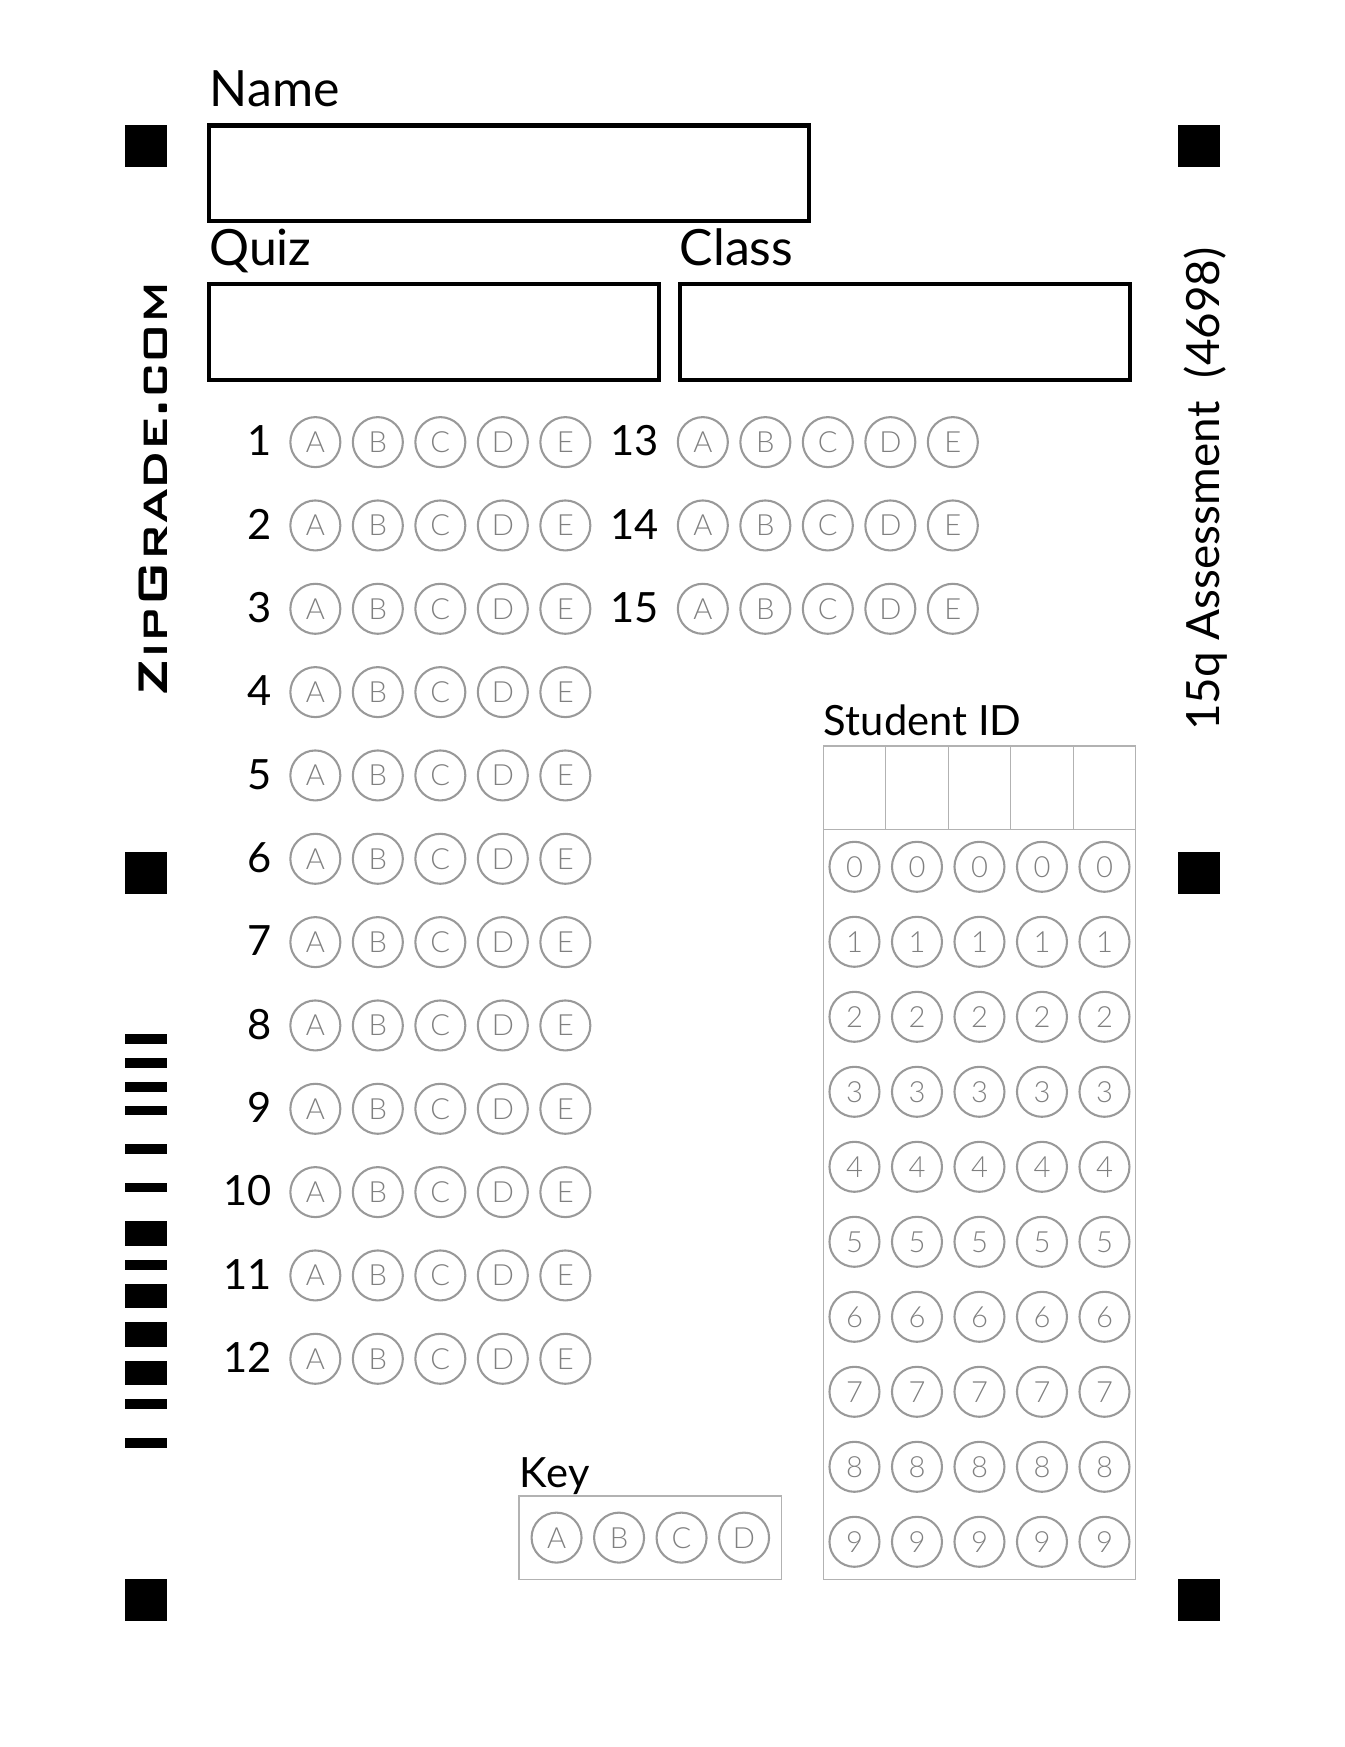
\includegraphics[width=4.3in]{scantron.png}};
      \fill (#1,#2) circle (0.25);
      \node[anchor=west] at (2,11.5) {\small \mytitle};
      %\fill[white] (6.8,8.3) rectangle (7.8,1.4);
      \node[fill=white] at (7.9,8.6) {\bf ZipGrade ID:};
    \end{tikzpicture}

  \end{flushright}
}

\renewcommand{\ku}{
    \begin{center}
        \begin{tabular}
          {p{1.25in}|p{1.5in}|p{1in}}
          \small Knowns/Unknowns    &
          \small  Plug \& Chug      & 
          \small Answer w/ Units \\
          &&\\[15em]
        \end{tabular}
      \end{center}
}

\begin{document}
\pagestyle{empty}



%%%%% TEST A %%%%%%%%
\begin{multicols}{2}
  \drawscantron{4.7}{1.8}

  \columnbreak

  \begin{align*}
    v &=f\lambda
  \end{align*}

  \paragraph{Problem 16} 
    What is the frequency of a wave with a wavelength of 7 meters and a speed of 17 m/s?
    \ku

  \paragraph{Problem 17} 
    What is the speed of a wave with frequency 300 Hz and wavelength 15 meters?
    \ku

\end{multicols}
\pagebreak

%%%%% TEST B %%%%%%%%
\begin{multicols}{2}
  \drawscantron{5.1}{1.8}

  \columnbreak

  \begin{align*}
    v &=f\lambda
  \end{align*}

  \paragraph{Problem 16} 
    What is the speed of a wave with frequency 350 Hz and wavelength 8 meters?
    \ku

  \paragraph{Problem 17} 
    What is the frequency of a wave with a wavelength of 13 meters and a speed of 53 m/s?
    \ku

\end{multicols}
\pagebreak

%%%%% TEST C %%%%%%%%
\begin{multicols}{2}
  \drawscantron{5.7}{1.8}

  \columnbreak

  \begin{align*}
    v &=f\lambda
  \end{align*}

  \paragraph{Problem 16} 
    What is the frequency of a wave with a wavelength of 12 meters and a speed of 39 m/s?
    \ku

  \paragraph{Problem 17} 
    What is the speed of a wave with frequency 300 Hz and wavelength 7 meters?
    \ku

\end{multicols}
\pagebreak

%%%%% TEST D %%%%%%%%
\begin{multicols}{2}
  \drawscantron{6.1}{1.8}

  \columnbreak

  \begin{align*}
    v &=f\lambda
  \end{align*}

  \paragraph{Problem 16} 
    What is the speed of a wave with frequency 250 Hz and wavelength 17 meters?
    \ku

  \paragraph{Problem 17} 
    What is the frequency of a wave with a wavelength of 9 meters and a speed of 94 m/s?
    \ku

\end{multicols}
\pagebreak




\end{document}